\documentclass[thesis]{subfiles}

\begin{document}

\OnlyInSubfile{\setcounter{chapter}{2}}

\chapter{Molecular simulations}
\startcontents[chapters]
\printpartialtoc

\section{Statistical thermodynamics}

Macroscopic methods such as the one I discussed in chapter~\ref{sec:macroscopic}
can provide understanding and allow us to predict behavior in some cases; they
are not always sufficiently precise to gain a complete understanding of the
phenomenon at play. In particular, as these methods describe the systems at the
macroscopic level, they don't take into account the individual atoms, and the
interactions between them. Put another way, they don't describe the
\emph{chemistry} of the system. Statistical thermodynamic is a tool that we can
use to bring together the microscopic description of matter and the macroscopic
behavior and characteristics of the system (pressure, temperature, \dots).

In this chapter, I will derive and recall some concepts from statistical
thermodynamics I used during my PhD. For a more in depth description of
statistical mechanics, I recommend the books of
\citeauthor{Tuckerman2010}\cite{Tuckerman2010}, or (in french)
\citeauthor{Diu1996}\cite{Diu1996}.

\subsection{Maxwell-Boltzmann statistics in canonical ensemble}

We will consider a molecular system containing $N$ individual atoms behaving as
classical particles with individual positions $\r_i$, masses $m_i$ and momentum
$\p_i$. Supposing that these particles are in some container of fixed volume
$V$, and at thermal equilibrium with a thermostat at temperature $T$, they
evolve in the canonical or $NVT$ ensemble. Finally, we will also assume that the
atoms in the system follow the Maxwell-Boltzmann statistics, \ie that the
probability that the system is in a state of internal energy $E_i$ is given by:
\[\mathcal{P}_i = \frac 1 Z e^{-\beta E_i}, \label{eq:maxwell-boltzmann}\]
where $\beta = 1 / k_B T$ with $k_B$ the Boltzmann constant and $Z$ is a
normalization constant called the \emph{partition function}. To be more precise,
particles would either follow Bose–Einstein statistics for Bosons (particles
with an integer spin, such as photons) or the Fermi–Dirac statistics for
Fermions (particles with half-integer spin, such as electrons or protons). But
as both Bose-Einstein and Fermi-Dirac statistics reduce to the Maxwell-Boltzmann
distribution when temperature is high enough, we will use this distribution
instead.

We define the state of a system by the values taken by all the positions $\r_i$
and all the momentum $\p_i$ of all the $N$ atoms in the system. The state of the
system is then defined by $6N$ variables, or a point in a vector space of $6N$
dimensions called the \emph{phase space}. In order to compute the energy of a
state, we will describe the interactions between the atoms by a potential energy
$\mathcal{V}(\r^N)$, independent of time. Then, we can compute the total energy
of a state using the classical Hamiltonian of the system:
\[H(\r^N, \p^N) = \sum_i^N \frac{\p_i^2}{2 m_i} + \mathcal{V}(\r^N);\]
where I use $\r^N$ and $\p^N$ as shorthand for the set of all positions
$\{\r_i\}$ and momentum $\{\p_i\}$ respectively.

The last element in equation~\eqref{eq:maxwell-boltzmann} we need to compute is
the partition function $Z$. In order to do so, we can note that the probability
for the system to be anywhere in the phase space $\Phi$ should be 1.
\[\iiint_\Phi \mathcal{P}_i = 1\]
\[Z = \frac{1}{h^{3N}} \iiint_\Phi e^{-\beta H(\r^N, \p^N)} \ \d\r^N \d\p^N\]
where the Planck constant $h$ is used as a normalization factor used to make
sure that $Z$ has the right dimension.

We can already compute at least a part of this integral by separating the
kinetic and potential energy terms in the Hamiltonian:
\[Z = \frac{1}{h^{3N}} \prod_i^{3N} \int e^{-\beta \frac{p_i^2}{2 m_i}} \ \d p_i \iiint_V e^{-\beta \mathcal{V}(\r^N)} \ \d\r^N \]
where the potential energy integral is over all the accessible volume. The
kinetic energy term is a product of Gaussian integrals, and gives us the
following expression for the partition function:
\[Z = \prod_i^{3N} \sqrt{\frac{2\pi m_i}{\beta h^2}} \iiint_V e^{-\beta \mathcal{V}(\r^N)} \ \d\r^N\]
$\lambda_i = \sqrt{\frac{\beta h^2}{2\pi m_i}}$ is the de Broglie thermal
wavelength for a particle with mass $m_i$, and is homogeneous to a distance. In
the following, I will be using $\Lambda^N$ for the product over all particles
$\prod_i^N \lambda_i^3$. This gives the final expression for the partition
function:
\[Z = \frac{1}{\Lambda^N} \iiint_V e^{-\beta \mathcal{V}(\r^N)} \ \d\r^N \label{eq:partition-function}\]

\subsubsection{Thermodynamic quantities from the partition function}

It is possible to use the knowledge of the partition function to compute some
of the macroscopic properties of our system. For examples, the internal energy
is the average value of the Hamiltonian:
\[U = \frac{1}{Z} \iiint_\Phi H e^{-\beta H} \]
If we express $H e^{-\beta H}$ as the partial derivative of $e^{-\beta H}$ with
respect to $\beta$ we get
\[U = \frac{1}{Z} \iiint_\Phi -\frac{\partial}{\partial \beta} e^{-\beta H} \]
\[U = \frac{-1}{Z} \frac{\partial}{\partial \beta} \iiint_\Phi e^{-\beta H} \]
\[U = \frac{-1}{Z} \frac{\partial Z}{\partial \beta}\]
Or equivalently
\[U = \frac{\partial \ln Z}{\partial \beta}\]

Using the same ideas, we can derive expressions\cite{Tuckerman2010} for the
entropy $S$ and the free energy $F$ using the partition function:
\[F = - \frac 1 \beta \ln Z\]
\[S = k_B \left[\ln Z + \beta \frac{\partial \ln Z}{\partial \beta} \right]\]

\subsubsection{Observables}

The probability for the system to be in a given state gives us the missing link
between microscopic and macroscopic properties of the system. We can express a
macroscopic observable property $A$ that we can also compute or measure at a
microscopic level using the the Maxwell-Boltzmann statistics:
\[A = \braket{A} = \iiint_\Phi P_i A_i.\]
The value of $A$ at a macroscopic level is the same value as the ensemble
average $\braket{A}$, which depends on both the value of the property in a given
macroscopic state $A_i$, and the probability of the system to be in this state.
Using equations~\eqref{eq:maxwell-boltzmann} and~\eqref{eq:partition-function}
together, we can express the average value for any observable property in the
canonical ensemble:
\[\braket{A} = \frac{\iiint_\Phi \d\r^N \d\p^N \; A(\r^N, \p^N) \ e^{-\beta H(\r^N, \p^N)}}{\iiint_\Phi \d\r^N \d\p^N \; e^{-\beta H(\r^N, \p^N)}}. \label{eq:observable-micro-macro}\]

\subsubsection{Sampling}

This theoretical approach to define macroscopic properties from microscopic data
is useless unless we can compute the integrals over the whole phase space $\Phi$
in~\eqref{eq:observable-micro-macro}. But computing this integral explicitly in
all but the simplest cases will prove difficult, as the phase space is a $6N$
dimensional vector space; and values for $N$ range from a few hundred all the
way up to Avogadro number. But in general a lot of states in the phase space are
not relevant when computing the integral, mainly because they have a too high
energy. So instead of computing the whole integral, we resort to only use a
finite number of samples in the phase space, which we try to pick as the most
relevant. In a semi-formal manner, we try to generate a set of points $\phi$
inside the phase space, such as
\[\braket{A} \approx \frac{\sum_\phi A(\r^N, \p^N) e^{-\beta H(\r^N, \p^N)}}{\sum_\phi e^{-\beta H(\r^N, \p^N)}}.\]

There are a few algorithms we can use to do this sampling and generate the set
$\phi$ of points we will use to compute a given property. I will discuss two of
them below: the Metropolis Monte Carlo (MC) method, and Molecular Dynamics (MD).
If we can get these algorithms to generate a set of states in the phase space
according to the Maxwell-Boltzmann probability, with the same state appearing
possibly more than once in the set, we can simplify the calculation of ensemble
average of observables even further. For a set of $m$ states indexed by
$\alpha$, the average reads as:
\[\braket{A} \approx \frac 1 m \sum_\alpha^m A(\r_\alpha^N, \p_\alpha^N).\]

\subsection{Other thermodynamic ensembles}

It is possible to show that in other thermodynamic ensembles there is a similar
probability distributions for the phase space, and the associated partition
function is also defined by the normalization of these probability distributions.

\paragraph{Isothermal-isobaric ensemble}
In the $NPT$ ensemble, the probability for the system to be in a state is given
by:
\[ \mathcal{P}_{NPT} = \frac{1}{\Delta} e^{-\beta \left[H(\r^N, \p^N) \ + \ PV\right]} \]
\[ \Delta = \frac{1}{\Lambda^N} \int \d V \iiint_V \d\r^N \; e^{-\beta \left[\mathcal{V}(\r^N) \ + \ PV\right]} \]

And the free energy is given by:
\[G = - \frac 1 \beta \ln \Delta.\]

\paragraph{Grand canonical ensemble}
In the $\mu VT$ ensemble, the probability for the system to be in a state is
given by:
\[ \mathcal{P}_{\mu VT} = \frac{1}{\Theta} e^{-\beta \left[H(\r^N, \p^N) \ - \ \sum_i \mu_i n_i \right]} \]
\[ \Theta = \frac{1}{\Lambda^N} \iint \d n_i \iiint_V \d\r^N \d\p^N \; e^{-\beta \left[\mathcal{V}(\r^N) \ - \ \sum_i \mu_i n_i \right]} \]

\paragraph{Osmotic ensemble}
In the osmotic ($N_\text{host} \ \mu \ PT$) ensemble, the probability for the system to be in
a state is given by:
\[ \mathcal{P}_{\mu VT} = \frac{1}{\zeta} e^{-\beta \left[H(\r^N, \p^N) \ + \ PV \ - \ \sum_i \mu_i n_i \right]} \]
\[ \zeta = \frac{1}{\Lambda^N} \int \d V \iint \d n_i \iiint_V \d\r^N \d\p^N \; e^{-\beta \left[\mathcal{V}(\r^N) \ + \ PV \ - \ \sum_i \mu_i n_i \right]} \]

\section{Computing energy of a molecular system}

\subsection{Quantum calculations}

In order to be able to use statistical thermodynamics we must compute the energy
$\mathcal{V}(\r^N)$ associated with a given configuration. The most generic way
to do so it to solve the Schrödinger equation for the system.

\fbox{MC quantique}
\fbox{HF}
\fbox{DFT}

But solving the Schrödinger equation is costly in term of computing time, and
thus impose a limit on both the time and length scale of systems we can study.
As of 2019, we can used DFT to study systems containing up to 1000 atoms on a
time scale of up to \SI{100}{ps}. While these numbers increased a lot in the
recent years due to improvements in software used for DFT and in computing
hardware, they are still many systems of interest that we can not study with
DFT. If the electronic density does no vary much across the subspace of phase
space we are interested in --- \ie no bond creation or breakage; no charge
transfer --- then using classical potentials or force fields can be a good
approximation of the real energy.

\subsection{Classical calculations: force fields}
\label{sec:classical-ff}

\TODO: pros and cons of this

If I had to define it, I would say that a force field is an educated guess on
the functional form of the energy of a system, decomposed as a sum of simple
terms. The usual decomposition is the following:
\[V(\r) = \sum_i \sum_j V_\text{pairs}^{ij} + \sum_\alpha V_\text{molecular}^\alpha + V_\text{coulomb} \]
where $V_\text{coulomb}$ is the Coulombic interaction between charged atoms,
$V_\text{molecular}$ represent the internal molecular energy and
$V_\text{pairs}$ represent the non-bonded pairs interactions. These terms are
often broken down even further. For example, the simplest form possible for
$V_\text{coulomb}$ is to use fixed point charges attributed to each atom during
the force field parametrization. If this is not enough to reproduce the
properties of the system of interest, we can use diffuse Gaussian charges
instead, or add atomic polarization. $V_\text{pairs}$ is used to reproduce both
the dispersion interaction and the Pauli repulsion between atoms at short
distance; and $V_\text{molecular}$ is usually decomposed over bonded
coefficients:
\[V_\text{molecular} = \sum_\text{bonds} V_\text{bond}(r) + \sum_\text{angles} V_\text{angle}(\theta) + \sum_\text{dihedrals} V_\text{dihedral}(\phi)\]
Each energy term only depends on the type of bonded atoms, and a single
parameter: the distance between the two atoms for bonds contributions; the
3-body angle for angles contributions; and the 4-body dihedral angle or out of
plane distance for dihedral angles contributions. These parameters are
illustrated in figure~\ref{fig:force-fields:molecular}.

\begin{figure}[ht]
    \centering
    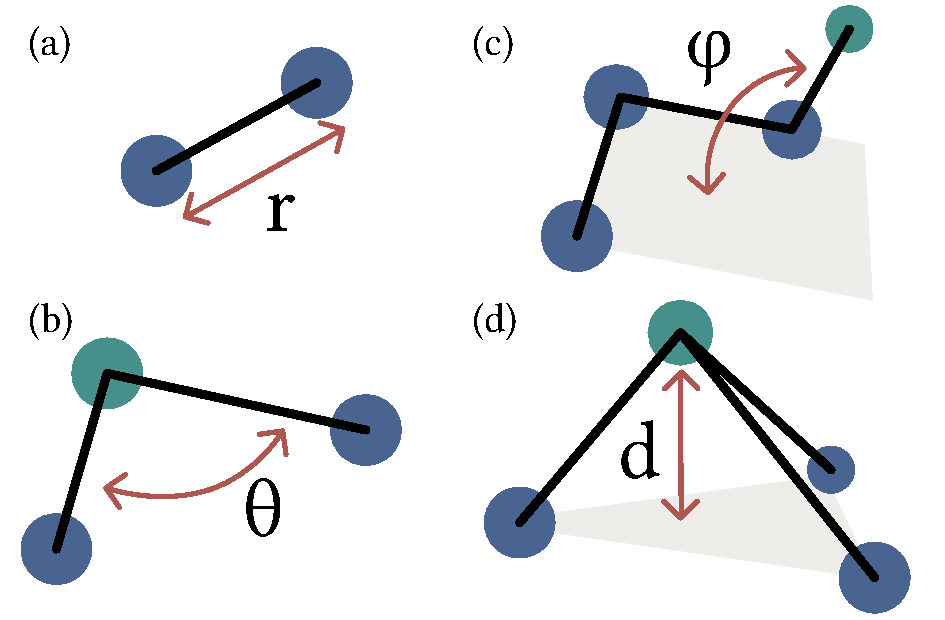
\includegraphics[width=.6\textwidth]{figures/images/molecular-ff}
    \caption{Definition of the parameters used to compute the energy of a
    molecular system with classical force field. (a) bond terms; (b) angle
    terms; (c) dihedral angles; (d) improper dihedrals/out of plane distance.}
    \label{fig:force-fields:molecular}
\end{figure}

\subsubsection{Typical functional forms used in force fields}

Their is no strict rule regarding which functional form can or can not be used
in a force field, so when creating a new force field we usually rely on
chemical sense as well as few physical laws to pick them. Here are a few well
known and widely used contributions in force fields.

\paragraph{Charges} If we choose to model atomic partial charges as point
charges, we can directly use the expression for Coulombic interactions, as a sum
over all pairs of charged atoms in the system:
\[ V(r_{ij}) = \frac{q_i q_j}{4 \pi \epsilon_0 r_{ij}}\]

\paragraph{Non-bonded pairs interactions} As we have seen, we use non-bonded
pairs interactions to reproduce both the Pauli repulsion between atoms at short
distances, and the dispersion attractive interaction at long distances. It can
be shown\cite{London1930} that the dispersion interaction can be developed in
the long distances approximation as:
\[ V_\text{dispersion} = -\frac{C_6}{r^6} + \frac{C_8}{r^8} - \frac{C_{10}}{r^{10}} + {\scriptstyle\mathcal{O}}\left(\frac{1}{r^{12}}\right) \]
where the $C_i$ coefficients have positive values. Most of the time, only the
term in $1/r^6$ is used, as it will have the largest contribution to the
resulting energy. There is however no simple mathematical expression for the
Pauli repulsion, so various schemes have been used.

The most prevalent one is the Lennard-Jones potential, which uses a repulsive
term proportional to $1/r^{12}$. In the early day of molecular simulation, this
allowed to save some computing time by squaring the already computed $1/r^6$ term.
\[V_\text{Lennard-Jones}(r) = 4 \ \epsilon \left[\left(\frac{\sigma}{r}\right)^{12} - \left(\frac{\sigma}{r}\right)^6\right]\]
Another commonly used form is the Buckingham potential, using an exponential
function for the repulsion:
\[V_\text{Buckingham}(r) = A \ e^{-B r} - \frac{C}{r^6}\]

\paragraph{Molecular interactions} The most common strategy for describing bonds
and angles is to consider only vibration of the bond length or the angle around
the equilibrium, and represent the energy of the bond/angle using the harmonic
approximation:
\[V_\text{harmonic}(r) = \frac 12 k \ (r - r_0)^2  \qquad\text{or}\qquad V_\text{harmonic}(\theta) = \frac 12 k \ (\theta - \theta_0)^2 \]

For dihedral angles, we often want to be able to reproduce the periodicity of
the associated energy, which leads to the following definition of the energy:
\[V_\text{torsion}(\phi) = \frac 12 E \left[1 + \cos(n \phi + \delta)\right] \]

\subsection{Energy evaluation tricks}

\fbox{cutoff? => Ewald}

\fbox{Restrictions}

\subsection{Force field parametrization}

All these functional forms have some kind of adjustable parameters that depends
on the types of the atoms participating in the pair; bond; or angle. For
example, when using Coulombic interactions, the charge carried by an atom is the
adjustable parameter. Both the equilibrium distance and the strength of the
spring depend on the two bonded atoms types in an harmonic bond.

=> parametrization, cf \ref{sec:classical-ff-parametrize}

\section{Metropolis Monte Carlo}
~

\subsection{Direct sampling of ensembles}
~

\subsection{Monte Carlo moves}
~

\subsection{Computing energy in Monte Carlo simulations}
~

\section{Molecular dynamics}
~
% We will assume that the atoms behave as classical point particles

\subsection{Integrators}
~

\subsection{Sampling other ensembles}
~

\section{Free energy methods}
~

\subsection{Umbrella sampling}
~

% WHAM

\OnlyInSubfile{\printbibliography}

\end{document}
